\documentclass[journal,12pt,twocolumn]{IEEEtran}

\usepackage{setspace}
\usepackage{gensymb}

\singlespacing


\usepackage[cmex10]{amsmath}

\usepackage{amsthm}

\usepackage{mathrsfs}
\usepackage{txfonts}
\usepackage{stfloats}
\usepackage{bm}
\usepackage{cite}
\usepackage{cases}
\usepackage{subfig}

\usepackage{longtable}
\usepackage{multirow}

\usepackage{enumitem}
\usepackage{mathtools}
\usepackage{steinmetz}
\usepackage{tikz}
\usepackage{circuitikz}
\usepackage{verbatim}
\usepackage{tfrupee}
\usepackage[breaklinks=true]{hyperref}

\usepackage{tkz-euclide}

\usetikzlibrary{calc,math}
\usepackage{listings}
    \usepackage{color}                                            %%
    \usepackage{array}                                            %%
    \usepackage{longtable}                                        %%
    \usepackage{calc}                                             %%
    \usepackage{multirow}                                         %%
    \usepackage{hhline}                                           %%
    \usepackage{ifthen}                                           %%
    \usepackage{lscape}     
\usepackage{multicol}
\usepackage{chngcntr}

\DeclareMathOperator*{\Res}{Res}

\renewcommand\thesection{\arabic{section}}
\renewcommand\thesubsection{\thesection.\arabic{subsection}}
\renewcommand\thesubsubsection{\thesubsection.\arabic{subsubsection}}

\renewcommand\thesectiondis{\arabic{section}}
\renewcommand\thesubsectiondis{\thesectiondis.\arabic{subsection}}
\renewcommand\thesubsubsectiondis{\thesubsectiondis.\arabic{subsubsection}}


\hyphenation{op-tical net-works semi-conduc-tor}
\def\inputGnumericTable{}                                 %%

\lstset{
%language=C,
frame=single, 
breaklines=true,
columns=fullflexible
}
\begin{document}


\newtheorem{theorem}{Theorem}[section]
\newtheorem{problem}{Problem}
\newtheorem{proposition}{Proposition}[section]
\newtheorem{lemma}{Lemma}[section]
\newtheorem{corollary}[theorem]{Corollary}
\newtheorem{example}{Example}[section]
\newtheorem{definition}[problem]{Definition}

\newcommand{\BEQA}{\begin{eqnarray}}
\newcommand{\EEQA}{\end{eqnarray}}
\newcommand{\define}{\stackrel{\triangle}{=}}
\bibliographystyle{IEEEtran}
\providecommand{\mbf}{\mathbf}
\providecommand{\pr}[1]{\ensuremath{\Pr\left(#1\right)}}
\providecommand{\qfunc}[1]{\ensuremath{Q\left(#1\right)}}
\providecommand{\sbrak}[1]{\ensuremath{{}\left[#1\right]}}
\providecommand{\lsbrak}[1]{\ensuremath{{}\left[#1\right.}}
\providecommand{\rsbrak}[1]{\ensuremath{{}\left.#1\right]}}
\providecommand{\brak}[1]{\ensuremath{\left(#1\right)}}
\providecommand{\lbrak}[1]{\ensuremath{\left(#1\right.}}
\providecommand{\rbrak}[1]{\ensuremath{\left.#1\right)}}
\providecommand{\cbrak}[1]{\ensuremath{\left\{#1\right\}}}
\providecommand{\lcbrak}[1]{\ensuremath{\left\{#1\right.}}
\providecommand{\rcbrak}[1]{\ensuremath{\left.#1\right\}}}
\theoremstyle{remark}
\newtheorem{rem}{Remark}
\newcommand{\sgn}{\mathop{\mathrm{sgn}}}
\providecommand{\abs}[1]{\left\vert#1\right\vert}
\providecommand{\res}[1]{\Res\displaylimits_{#1}} 
\providecommand{\norm}[1]{\left\lVert#1\right\rVert}
%\providecommand{\norm}[1]{\lVert#1\rVert}
\providecommand{\mtx}[1]{\mathbf{#1}}
\providecommand{\mean}[1]{E\left[ #1 \right]}
\providecommand{\fourier}{\overset{\mathcal{F}}{ \rightleftharpoons}}
%\providecommand{\hilbert}{\overset{\mathcal{H}}{ \rightleftharpoons}}
\providecommand{\system}{\overset{\mathcal{H}}{ \longleftrightarrow}}
	%\newcommand{\solution}[2]{\textbf{Solution:}{#1}}
\newcommand{\solution}{\noindent \textbf{Solution: }}
\newcommand{\cosec}{\,\text{cosec}\,}
\providecommand{\dec}[2]{\ensuremath{\overset{#1}{\underset{#2}{\gtrless}}}}
\newcommand{\myvec}[1]{\ensuremath{\begin{pmatrix}#1\end{pmatrix}}}
\newcommand{\mydet}[1]{\ensuremath{\begin{vmatrix}#1\end{vmatrix}}}
\numberwithin{equation}{subsection}
\makeatletter
\@addtoreset{figure}{problem}
\makeatother
\let\StandardTheFigure\thefigure
\let\vec\mathbf
\renewcommand{\thefigure}{\theproblem}
\def\putbox#1#2#3{\makebox[0in][l]{\makebox[#1][l]{}\raisebox{\baselineskip}[0in][0in]{\raisebox{#2}[0in][0in]{#3}}}}
     \def\rightbox#1{\makebox[0in][r]{#1}}
     \def\centbox#1{\makebox[0in]{#1}}
     \def\topbox#1{\raisebox{-\baselineskip}[0in][0in]{#1}}
     \def\midbox#1{\raisebox{-0.5\baselineskip}[0in][0in]{#1}}
\vspace{3cm}
\title{EE5609 Assignment 4}
\author{Abhishek Thakur}
\maketitle
\newpage
\bigskip
\renewcommand{\thefigure}{\theenumi}
\renewcommand{\thetable}{\theenumi}
\begin{abstract}
This document contains the solution of geometry through linear algebra.
\end{abstract}
Download latex and python codes from 
\begin{lstlisting}
https://github.com/abhishekt711/EE5609/tree/master/Assignment_4
\end{lstlisting}
%
\section{Problem}
Find the smaller area enclosed by the circle  $\vec{x}\vec{x}^T=4$ and the line $\myvec{1 & 1} \vec{x}=2$.
\section{Explanation}
General equation of circle is 
\begin{align}
{\vec{x}^T\vec{x}} + 2\vec{u}^T\vec{x} + f = 0 \label{eq1}\\
 \norm{\vec{x}}^2 + 2\vec{u}_1^T\vec{x} + f_1 = 0\label{eq2}\\
 {\vec{x}^{T}\vec{x}}-4=0 \label{eq3}\\
 \vec{u_1}=\myvec{0\\0}\label{eq4}\\
 f_1=-4\label{eq5}\\
\vec{O_1}=\myvec{0\\0}\label{eq6}\\
r=\sqrt{\vec{c}^{T}\vec{c}-f} = \sqrt{4}\label{eq7}\\
    \implies \boxed{r=2} \label{eq8}
 \end{align}
From equation \eqref{eq8}, the point at which circle touches $x$-axis is \myvec{-2\\0} and \myvec{2\\0}.\\
The direction vector of the given line $\myvec{1&1}\vec{x}=2$ is $\myvec{-1\\1}$.\\

\begin{figure}[h!]
	\centering
	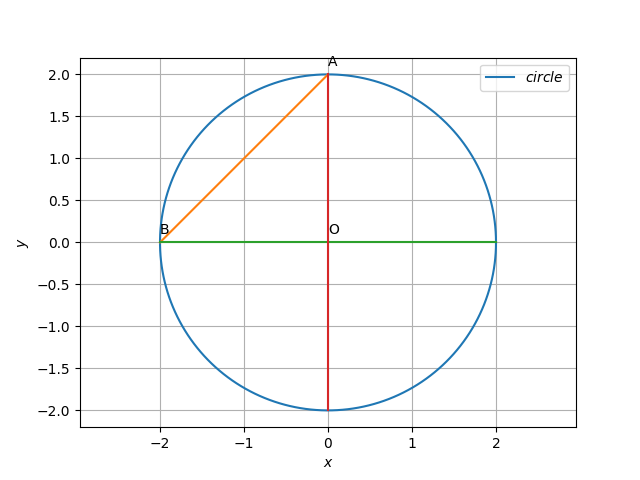
\includegraphics[width=\columnwidth]{circle.png}
	\caption{Smaller area enclosed by line and circle}
	\label{eq:myfig}
\end{figure}

To find point $\vec{A}$ and $\vec{B}$,
The parametric form of line is,
\begin{align}
    \vec{A} = \vec{q}+\lambda\vec{m}\label{eq9}\\
            = \myvec{1\\1}+\lambda\myvec{-1\\1}\label{eq10}\\
    \lambda^2 = \frac{-f_1-\norm{\vec{q}}^2}{\norm{\vec{m}}^2}\label{eq11}\\
                = \frac{4-2}{2} = 1\label{eq12}\\
    \implies \lambda = \pm{1} \label{eq13}\\
    \vec{A} = \myvec{0\\2}\quad \vec{B} = \myvec{-2\\0}\label{eq14}
\end{align}
Smaller area enclosed by circle and line $\bf{AB}$ is:\\
 Area = (Area of circle in 2nd Quadrant) - (Area of right triangle formed by line AB, X and Y axis)
 \begin{align}
Area=\frac{\pi\theta_1}{360}r^2-\frac{1}{2}\times2\times2\label{eq15}\\
=\frac{90}{360}\pi\times2^2-2\label{eq16}\\
=\pi-2\label{eq17}
\end{align}
Hence, the smaller area enclosed by the circle  $\vec{x}\vec{x}^T=4$ and the line $\myvec{1 & 1} \vec{x}=2$ is $\pi-2$
\end{document}